\section{Scenario}
\textcite{zhang2019scenario} use an example of a small \gls{spa} titled "Math for kids", which generates simple math addition problems and keeps track of a small statistic, which includes the number of correctly and incorrectly answered problems. The same application has been implemented and extended in Vue.js and will be used to display the capabities of the interaction diagram and scenario generation application.
%TODO rename section "Simple Application"? "Basic capabilities?" 
%"the morning is wiser than the evening" '\parencite{ aafanasyev_vasilisa_1997}

\section{Math for Kids}

\begin{figure}[H]
    \centering
    \begin{subfigure}[b]{0.45\textwidth}
         \centering
         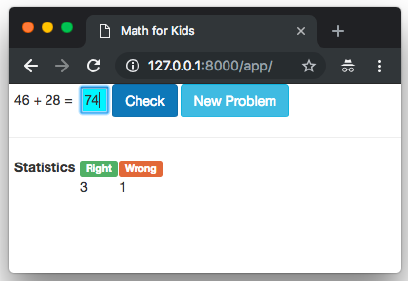
\includegraphics[width=0.45\textwidth]{images/math_for_kids_zhang.png}
         \caption{Math for Kids in AngularJS by \textcite{zhang2019scenario}}
         \label{fig:evaluation_math_kids_zhang}
    \end{subfigure}\hfill%
    \begin{subfigure}[b]{0.45\textwidth}
        \centering
        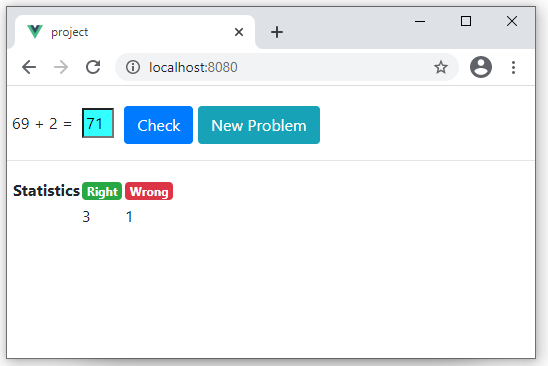
\includegraphics[width=0.45\textwidth]{images/math_for_kids_own.png}
        \caption{Own implementation of Math for Kids in Vue.js}
        \label{fig:evaluation_math_kids_own}
    \end{subfigure}\hfill%
\end{figure}

The source code can be found in \code{resources/test-files/test.vue} and also in \ref{appendix:math_kids_basic_source_code}.
\begin{figure}[H]
    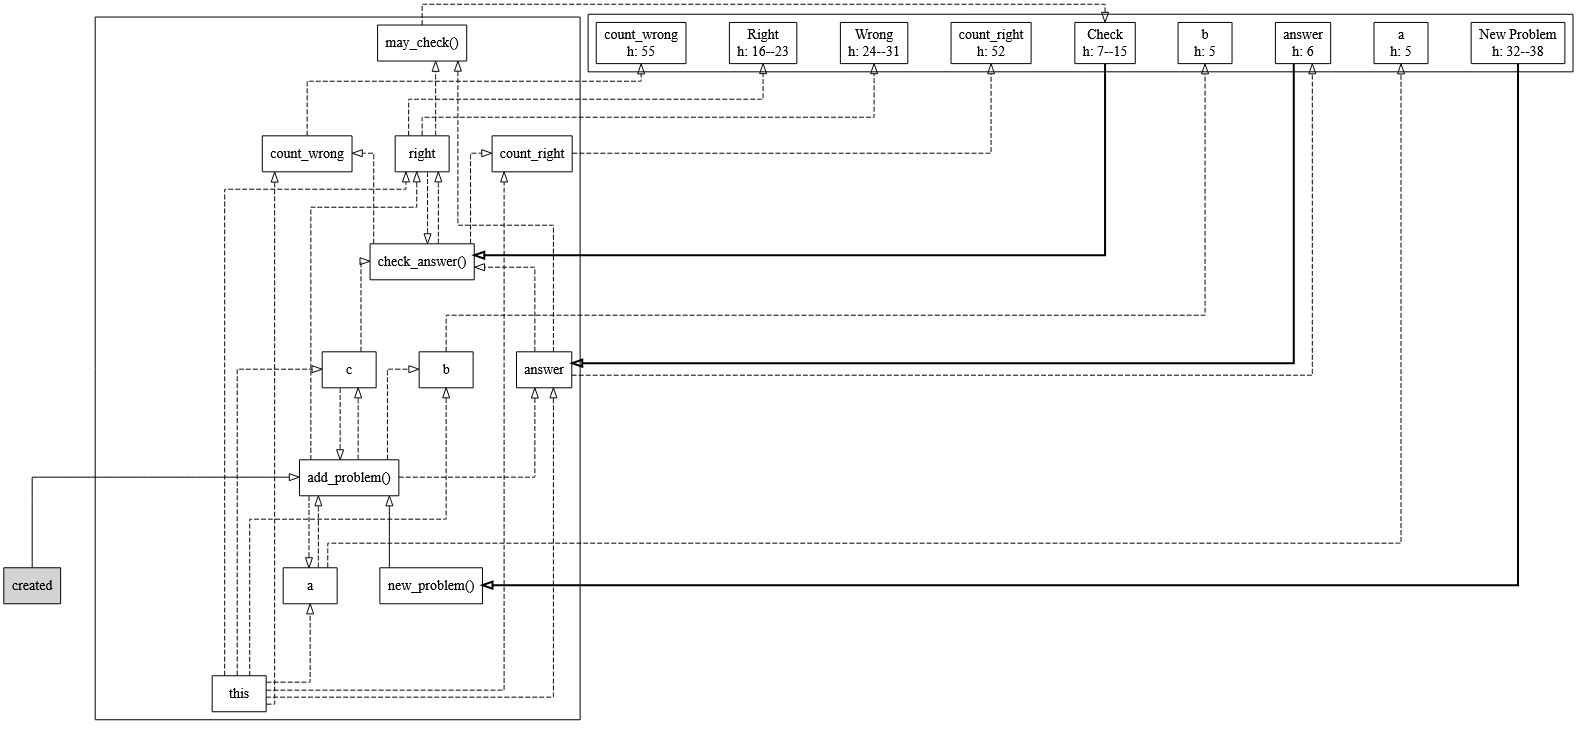
\includegraphics[width=\textwidth]{images/diagram_own_math_kids.png}
     \caption{Math for Kids in Vue.js generated interaction diagram }
     \label{fig:math_for_kids_own_interaction_diagram}
\end{figure}

\begin{figure}[H]
    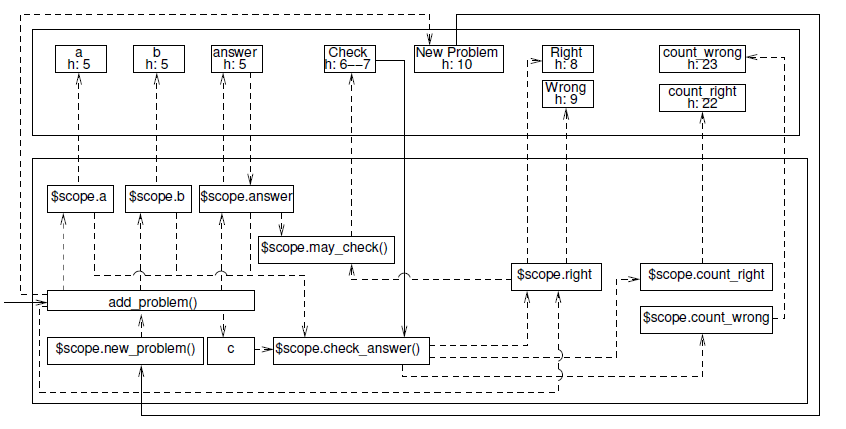
\includegraphics[width=\textwidth]{images/interaction_diagram_zhang.png}
     \caption{Math for Kids in AngularJS interaction diagram by \textcite{zhang2019scenario}}
     \label{fig:math_for_kids_zhang_interaction_diagram}
\end{figure}

When comparing the generated diagram\ref{fig:math_for_kids_own_interaction_diagram} to the original by \textcite{zhang2019scenario} \ref{fig:math_for_kids_zhang_interaction_diagram} there are some differences.

Due to different modelling there is a \code{this} vertex and connections from it to top level variables, which does not exist in the diagram by \textcite{zhang2019scenario}. In the generated diagram there is an edge of type 'event' between the \textit{answer} tag and \textit{answer} property. This is due to the way that two-way bindings were decided to be represented.

There are two differences between the \textit{add\_problem} node in the generated diagram and the one by \textit{zhang2019scenario}.
In \textcite{zhang2019scenario} there is an edge from
the \textit{add\_problem} method to the \textit{New Problem} tag, which is missing in the own generated version. This seems like a mistake in \parencite{zhang2019scenario}, since this edge should not exist.

The other difference is that in \parencite{zhang2019scenario} there is no edges from \textit{add\_problem} to \textit{right} (write relation), however there should be, 
inside \textit{add\_problem} \code{this.right = undefined}.

\begin{lstlisting}
l(created) -> a, b, answer, Check, Right, Wrong
l(answer) -> answer, Check
l(Check) -> Right, Wrong, Check, count_right, count_wrong
l(New Problem) -> a, b, answer, Check, Right, Wrong
\end{lstlisting}

The generated reaction based on the graph differ for $l(created)$, all other sets are exactly the same as the ones by \textcite{zhang2019scenario} (albeit in different order). This may stem from the fact that the edges of \textit{add\_problem} to \code{\$scope.right} is missing in \parencite{zhang2019scenario}, however it is later correctly factored in $l(New Problem)$.

\textcite{zhang2019scenario} define $l(add_problem())$ 
(the equivalent of $l(created)$) as $l(add_problem() = 
{a, b})$ where it should be 
$l(add_problem() = {Check, Right, Wrong, a, b, answer })$ since the answer property is updated based on the diagram. 

One could argue, that the version in \parencite{zhang2019scenario} is correct, since $answer$ is set to $undefined$, which is the same as the initial value of the variable, so it would not trigger an update as part of the \code{init} method. The interaction diagram generator does not perform this check. If $l(add_problem())$ were to be called later in the application (when the $New Problem$ button is clicked) it would indeed set a new value to $answer$, which is correctly reflected by \textcite{zhang2019scenario}.


\subsection{Scenarios}
Gherkin scenarios of up to 4 actions are generated, which can be seen in the following figures. The program outputs the scenarios as plain text to the console, but here they are displayed in a nicer way. The caption of each figure is an example of how a text could be generated based on the template scenario output by the application.

%TODO cite and explain  this in first section and ref from here
Some scenarios seem a bit repetitive, but it is up to \textit{The Three Amigos} - The product owner, tester and developer \parencite{cucumber_amigos} to decide which templates to discard. Since interaction diagrams model what \textit{might} be updated, it will probably be reasonable to discard some scenarios. The fact that everything which might get updated can also be leveraged in another way - negative criteria can be definied (assert tag/component $X$ did not change).
%TODO play around with subfigure alignment, there be
%https://tex.stackexchange.com/questions/333249/controlling-subfigure-captions-and-subfigure-placement
\begin{figure}[H]
    \label{fig:eval_scenarios_0}
    \caption{Gherkin scenarios templates and sample human written scenarios based on the templates }
    \centering
    \begin{subfigure}[b]{0.48\textwidth}
         \centering
         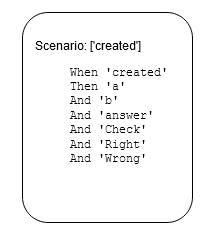
\includegraphics[width=0.48\textwidth]{images/scenarios_1.png}
         \caption{Scenario: initialization. When the application is created, then 'a' and 'b' should show random numbers and 'Check' should be disabled and 'Right' and Wrong should be invisible.}
    \end{subfigure}\hfill%
    \begin{subfigure}[b]{0.48\textwidth}
        \centering
        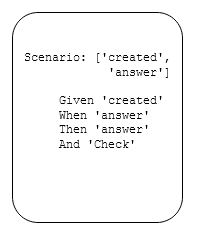
\includegraphics[width=0.48\textwidth]{images/scenarios_2.png}
        \caption{Scenario: typing an answer. Given the application has been created, when I type an answer then 'answer' should display it and 'Check' should be enabled.}
    \end{subfigure}\hfill%
    \begin{subfigure}[b]{0.48\textwidth}
        \centering
        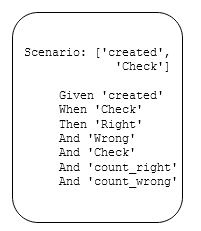
\includegraphics[width=0.48\textwidth]{images/scenarios_3.png}
        \caption{Scenario: clicking on check without typing an answer. Given the application has been created, when I click 'Check' then 'Right' and 'Wrong' should be invisible and 'count\_right' and 'count\_wrong' should have the same values and 'Check' should be disabled. }
   \end{subfigure}\hfill%
   \begin{subfigure}[b]{0.48\textwidth}
    \centering
    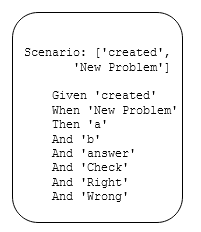
\includegraphics[width=0.48\textwidth]{images/scenarios_4.png}
    \caption{Scenario: obtaining a new problem at application start. Given the application has been created, when I click 'New Problem' then 'a' and 'b' should have random values and 'answer' should be empty and 'Check' should be disabled and 'Right' and 'Wrong' should be invisible.}
\end{subfigure}\hfill%
\end{figure}

\begin{figure}[H]\ContinuedFloat
    \centering
    \label{fig:eval_scenarios}
  
\begin{subfigure}[b]{0.48\textwidth}
    \centering
    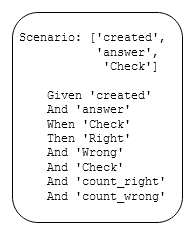
\includegraphics[width=0.48\textwidth]{images/scenarios_5.png}
    \caption{Scenario: checking my answer. Given the application has been created and 'answer' contains my answer, when I click 'Check' then 'Right' should be visible if the answer was right 'Wrong' should be visible if the answer was wrong and 'Check' should be disabled and 'count\_right' should be incremented by one if the answer was right and 'count\_wrong' should be incremented by one if the answer did not change. }
\end{subfigure}\hfill%
\begin{subfigure}[b]{0.48\textwidth}
    \centering
    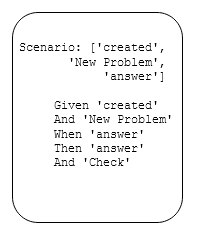
\includegraphics[width=0.48\textwidth]{images/scenarios_6.png}
    \caption{Scenario: typing an answer to a new problem. Given the application has been created and a new problem was obtained, when I type an answer then 'answer' should display it and 'Check' should be enabled.}
\end{subfigure}\hfill%
\begin{subfigure}[b]{0.48\textwidth}
    \centering
    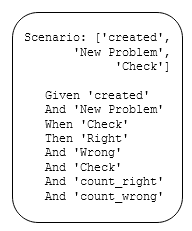
\includegraphics[width=0.48\textwidth]{images/scenarios_7.png}
    \caption{Scenario: requesting a new problem and clicking on check without answering it. Given the application has been created and I requested a new problem, when I click 'Check' then 'Right' and 'Wrong' should be invisible and 'count\_right' and 'count\_wrong' should have the same values and 'Check' should be disabled. }
\end{subfigure}\hfill%
\begin{subfigure}[b]{0.48\textwidth}
    \centering
    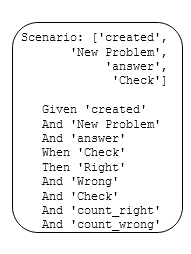
\includegraphics[width=0.48\textwidth]{images/scenarios_8.png}
    \caption{Scenario: requesting a new problem, answering it and checking my answer. Given the application has been created and I requested a new problem and answered it, when I click 'Check' then 'Right' should be visible if the answer was right 'Wrong' should be visible if the answer was wrong and 'Check' should be disabled and 'count\_right' should be incremented by one if the answer was right and 'count\_wrong' should be incremented by one if the answer did not change. }
\end{subfigure}\hfill%

\end{figure}

\section{Lists and Computed Properties}

\ref{fig:eval_image_list_complex} shows an extension to the Math for Kids application. The full source code can be found it \ref{appendix:math_kids_extended_source_code}

The application now displays past problems in a list, randomly generates either a subtraction or addition problem, and also keeps tracks of statistics separated by problem type and includes and additional accuracy statistic.

\begin{figure}[H]
    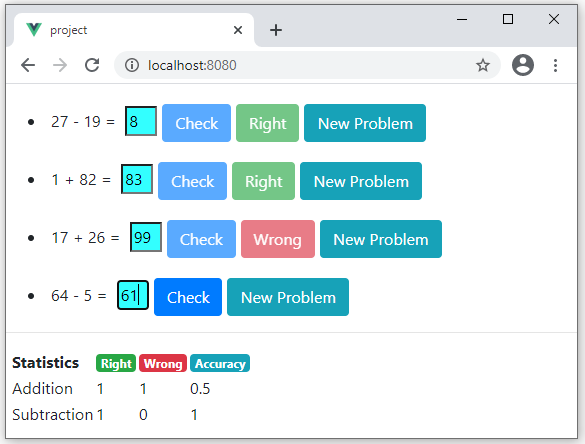
\includegraphics[width=\textwidth]{images/math_for_kids_own_complex.png}
     \caption{Math for Kids in Vue.js including subtraction problems, more precise statistics and display of past problems }
     \label{fig:eval_image_list_complex}
\end{figure}

\ref{fig:diagram_list_complex} shows the interaction diagram for the application, which looks more complex, but it is still possible to focus on specific components and see how they affect/are affected by others. 

The two vertices for the computed properties \textit{accuracy\_sub} and \textit{accuracy\_add} correctly directly depend on \textit{count\_right\_sub}, \textit{count\_wrong\_sub} and \textit{count\_right\_add}, \textit{count\_wrong\_add} respectively.

By looking at the reactions, one can observe that based on which of the mutually exclusive Check buttons is clicked on, either the substituting or addition related properties are updated. 

This example includes a bit of engineering - more realistically there would a single button, which checks inside the bound method which should be updated, however the application would not be able to be differentiate them in this case, since if statements inside methods are not supported.

This differentiation is also evident in the generated Gherkin scenario templates. 

All generated scenarion templates up to 4 actions can be seen in  \ref{appendix:math_kids_extended_scenarios}

\begin{lstlisting}
l(problems[i].answer) -> problems[i].answer, Check, Check
l(Check) -> Right, Wrong, Check, Check, count_right_add, accuracy_add, count_wrong_add
l(Check) -> Right, Wrong, Check, Check, count_right_sub, accuracy_sub, count_wrong_sub
l(New Problem) -> problems[i].a, +, -, Check, Check, problems[i].b, problems[i].answer, Right, Wrong
l(created) -> problems[i].a, +, -, Check, Check, problems[i].b, problems[i].answer, Right, Wrong
\end{lstlisting}

\begin{figure}[H]
    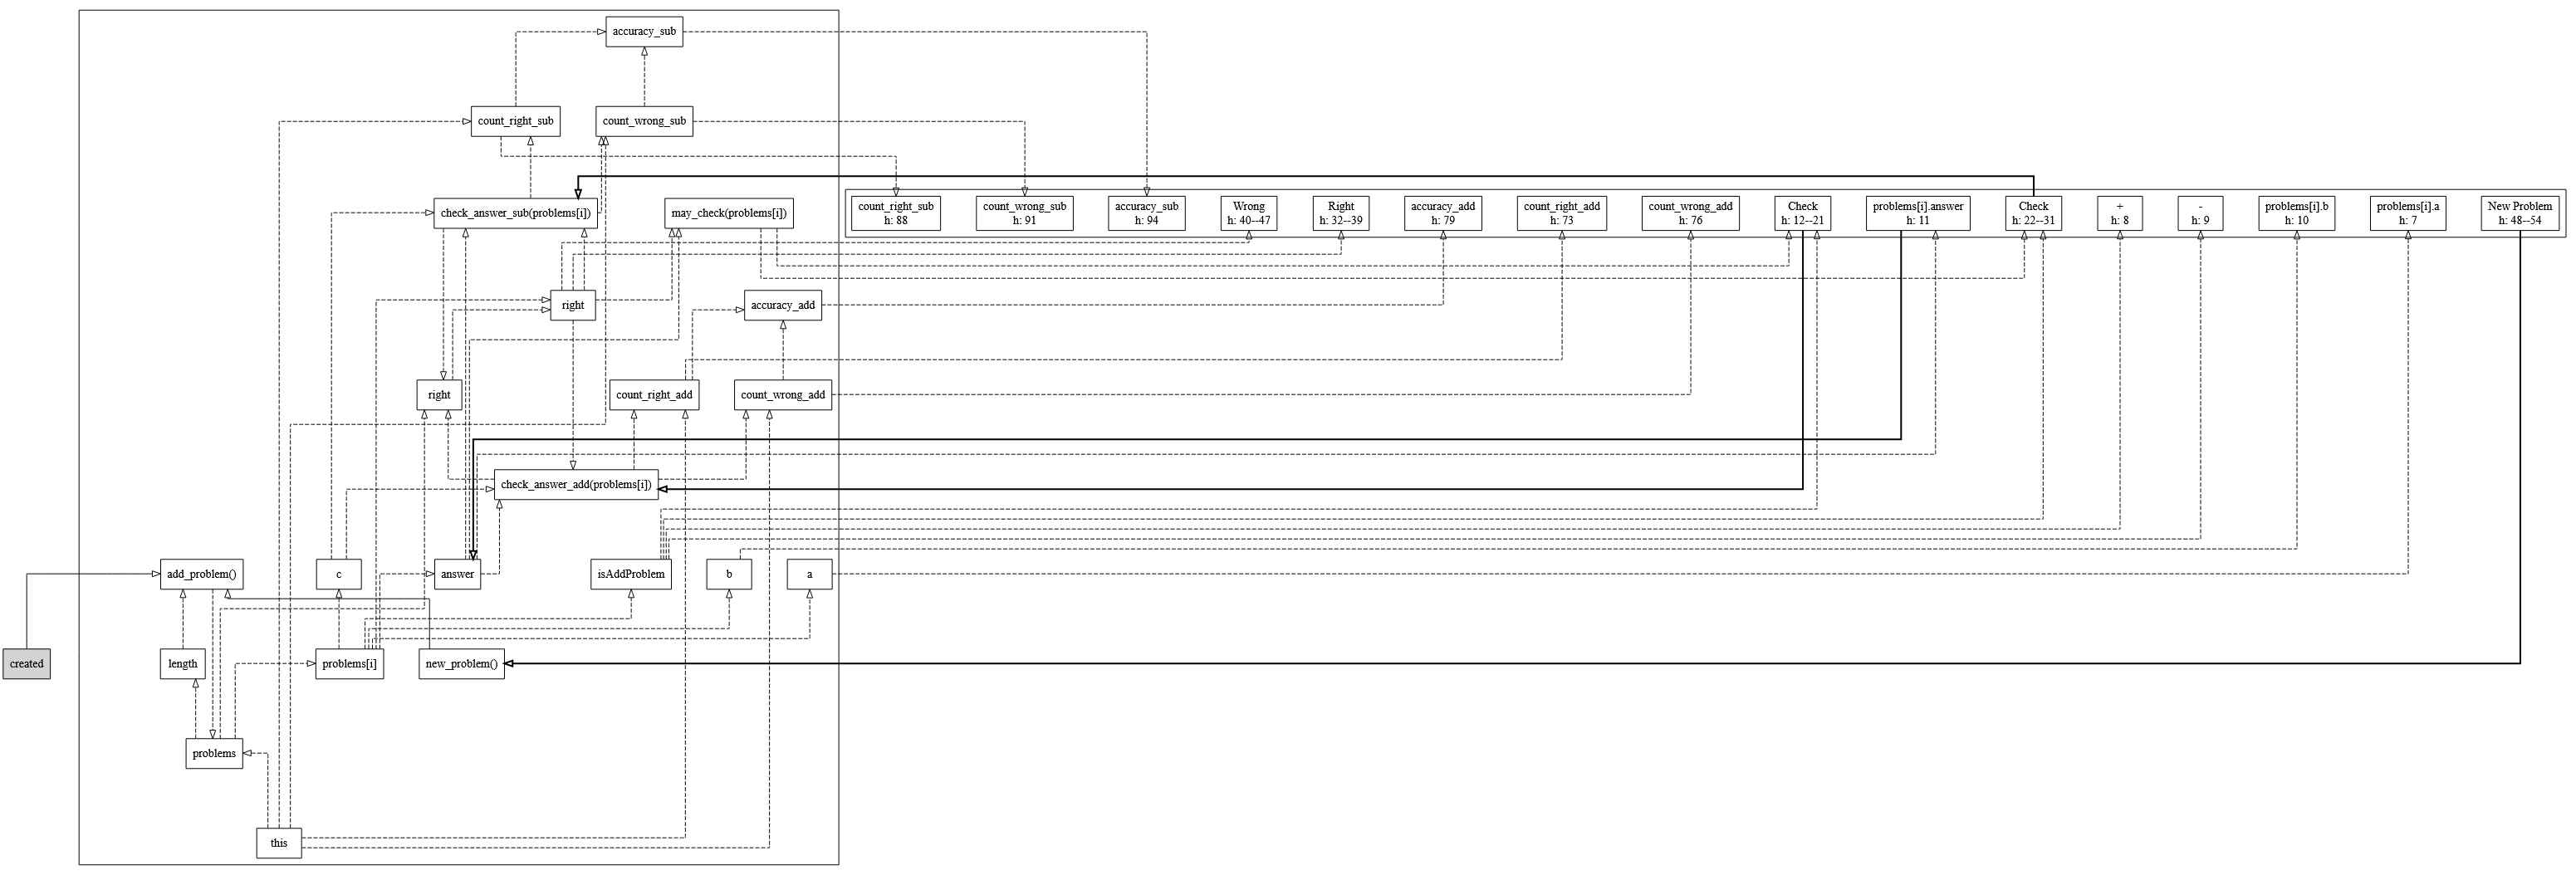
\includegraphics[width=\textwidth]{images/diagram_list_add_sub.png}
     \caption{Generated interaction diagram for Math for Kids including subtraction in Vue.js}
     \label{fig:diagram_list_complex}
\end{figure}


%TODO example to showcase list properties and multiple specific updates?

%TODO double check scenarios generated


%2. example with lists
%3. complex list(add, sub) with focus on updates


%TODO nah, noneed so formal

%example a bit engineered


%TODO link to https://github.com/KarakoA/vuejs-example and say examples can be deployed there